%%
%% This is file `article1.tex', % generated with the docstrip utility.
%%
%% The original source files were:
%%
%% dms.dtx  (with options: `article') % Example TeX file for the documentation %
%of the jurabib package % Copyright (C) 1999, 2000, 2001 Jens Berger % See
%dms.ins  for the copyright details.
%% 
%%% ====================================================================
%%%  @LaTeX-file{ %%     filename        = "dms.dtx", %%     author    =
%"Nicolas Beauchemin, Damien Rioux-Lavoie, Victor Fardel, Jonathan Godin", %%
%copyright = "Copyright (C) 2000 , DMS %%                  all rights reserved.
%Copying of this file is %%                  authorized only if either: %%
%(1) you make absolutely no changes to your copy, %%                  including
%name; OR %%                  (2) if you do make changes, you first rename it %%
%to some other name.", %%     address   = "Département de Mathématiques et de
%Statistique", %%     telephone = "514-343-6705", %%     FAX       =
%"514-343-5700", %%     email     = "aide@dms.umontreal.ca (Internet)", %%
%keywords  = "latex, amslatex, ams-latex, theorem", %%     abstract  = " Ce
%fichier est un package conçu pour être %%                  utilisé avec la
%version de LaTeX2e 1995/06/01. Il %%                  est prévue pour la classe
%``amsbook''. Il en %%                  modifie le format des pages, l'entête
%des %%                  sections, etc, afin d'être  conforme au modèle de %%
%mémoire de maîtrise de l'Université de %%                  Montréal. Finalement
%ce fichier est grandement %%                  inspiré du fichier
%amsclass.dtx.", %%     docstring = "The checksum field contains: CRC-16
%checksum, %%                  word count, line count, and character count, as
%%%                  produced by Robert Solovay's checksum utility."}
%%%  ====================================================================

%% To change chapter header dynamically from french to english, use
%%\entetedynamique
\setcounter{corA}{0} % Pour recommancer à compter les def,
                     % theo, etc. à partir de 1
 % Pour écrire un article en français
%% \francais
 % Pour écrire un article en anglais
\anglais
%% NOTE: La plupart des macros ont un nom en anglais. % P.ex. \adresse et
%\address fonctionnent et sont équivalents. % \revue=\journal % \auteur=\author
%% \titre=\title

\doublespacing

%% Les contributions apparaîtront habituellement après % \maketitle (voir un peu
%plus bas). Selon les goûts, il est % possible de mettre les contributions %
%avant la page titre de l'article, simplement en les écrivant % directement ici.
%Par exemple :
 % \cleardoublepage \pdfbookmark[chapter]{Contributions}{contrib1} % Remplacer
 % par contrib2 pour l'article 2 etc. {\bfseries\Large\noindent Contributions de
 % <mon nom> et rôle joué par les coauteurs} J'ai contribué en...
 %
 % Le rôle des coauteurs a été de...

%% Nom de la revue de publication
\revue{Methods in Ecology and Evolution and is available at https://doi.org/10.1111/2041-210X.14228}
\article{Graph embedding and transfer learning can help predict potential species interaction networks despite data limitations}\label{Perspectives}
%% On peut se référer aux numéros de chapitre ou d'article comme suit. % Si on
%fait % \label{chap:article1}, % alors \ref{chap:article1} donnera le numéro du
%chapitre. On peut ensuite faire % \labelart{art:article1} % et alors
%\ref{art:article1} donnera le numéro d'article. % Par exemple, si cette article
%est le premier article et le deuxième chapitre, % alors si on écrit % Voir le
%chapitre~\ref{chap:article1} (l'article~\ref{art:article1}). % deviendra % Voir
%le chapitre 2 (l'article 1). % Si on veut écrire « premier article » au lieu «
%article 1 », on peut % simplement faire % \ordinal{\ref{art:article1}}~article
%% devient première article % ou % \Ordinal{\ref{art:article1}}~article  %
%devient Première article (avec la majuscule) % Si on est en mode \anglais,
%\ordinal écrire first, second,...

%%%%%%%%%%%%%%%%%%%%%%%%%%%%%%%%%%%%%%%%%%%%%%%%%%%%%%%%%%%%%%%
%%%%%%%%%%%%%%%%%     Contribution     %%%%%%%%%%%%%%%%%%%%%%%% %%%%%%%%%%%%%%%%
%(lire attentivement) %%%%%%%%%%%%%%%%%%%%%%%%
%%%%%%%%%%%%%%%%%%%%%%%%%%%%%%%%%%%%%%%%%%%%%%%%%%%%%%%%%%%%%%%
 % Contribution(s) peronnelle(s) à l'article et rôle joué par tous les
 % coauteur·e·s
 %
 % Nécessaire seulement lorsque vous n'êtes pas seul·e auteur·e. Les
 % contributions peuvent apparaître ailleur dans la thèse. Si \contributions est
 % laissé vide (p.ex. si vous effacez celui ci-bas), aucune contributions ne
 % seront générées sur la page titre de l'article. Vous pouvez alors mettre un
 % \newpage si vous souhaitez que les résumé et abstract soient sur la page
 % suivante.
 %
 % REMARQUE : À peu près toutes les constructions \LaTeX\ sont permises dans les
 % contributions.
 %
 % La commande admet une option [<entête>]
\contributions%[Mes contributions et le rôle des coauteurs]
{ 

TP and TS designed the study and edited the manuscript for submission. TS performed the analysis and wrote the manuscript. All authors contributed to the article and approved the submitted version.\\[1cm]
}

%%% INFORMATIONS POUR LA PAGE TITRE
 % Premier auteur·e et adresse

\auteur{Tanya Strydom}
\adresse{Département de Sciences Biologiques, Université de Montréal, Montreal, QC, Canada\\ Québec Centre for Biodiversity Sciences, Montreal, QC, Canada}
\auteur{Salomé Bouskila}
\adresse{Département de Sciences Biologiques, Université de Montréal, Montreal, QC, Canada\\ Québec Centre for Biodiversity Sciences, Montreal, QC, Canada}
\auteur{Francis Banville}
\adresse{Département de Sciences Biologiques, Université de Montréal, Montreal, QC, Canada\\
Université de Sherbrooke, Sherbrooke, Canada\\
Québec Centre for Biodiversity Sciences, Montreal, QC, Canada}
\auteur{Ceres Barros}
\adresse{Department of Forest Resources Management, University of British Columbia, Vancouver, BC, Canada}
\auteur{Dominique Caron}
\adresse{McGill University, Montréal, Canada\\ Québec Centre for Biodiversity Sciences, Montreal, QC, Canada}
\auteur{Maxwell J. Farrell}
\adresse{Department of Ecology \& Evolutionary Biology, University of Toronto, Toronto, ON, Canada}
\auteur{Marie-Josée Fortin}
\adresse{Department of Ecology \& Evolutionary Biology, University of Toronto, Toronto, ON, Canada}
\auteur{Benjamin Mercier}
\adresse{Université de Sherbrooke, Sherbrooke, Canada\\
Québec Centre for Biodiversity Sciences, Montreal, QC, Canada}
\auteur{Laura Pollock}
\adresse{McGill University, Montréal, Canada\\ Québec Centre for Biodiversity Sciences, Montreal, QC, Canada}
\auteur{Rogini Runghen}
\adresse{Centre for Integrative Ecology, School of Biological Sciences, University of Canterbury, Canterbury, New Zealand}
\auteur{Giulio V. Dalla Riva}
\adresse{School of Mathematics and Statistics, University of Canterbury, Christchurch, New Zealand}
\auteur{Timothée Poisot}
\adresse{Département de Sciences Biologiques, Université de Montréal, Montreal, QC, Canada\\ Québec Centre for Biodiversity Sciences, Montreal, QC, Canada}
%

\maketitle

\begin{resume}{réseaux écologiques, intégration de réseaux, apprentissage par transfert, macroécologie de réseau} 1. Les métawebs (réseaux d'interactions potentielles au sein d'un pool d'espèces) constituent une abstraction puissante pour comprendre comment sont structurés les réseaux d'interactions d'espèces à grande échelle.\\
2. Étant donné que les métawebs sont généralement exprimés à de grandes échelles spatiales et taxonomiques, leur assemblage est un processus fastidieux et coûteux ; les méthodes prédictives peuvent aider à contourner les limitations liées aux carences des données, en fournissant une première approximation des métawebs.\\
3. Une façon d'améliorer notre capacité à prédire les métawebs consiste à maximiser les informations disponibles en utilisant des graphiques intégrés, par opposition à une liste exhaustive des interactions entre espèces. L'intégration de graphes est un domaine émergent de l'apprentissage automatique qui recèle un grand potentiel de problèmes écologiques.\\
4. Ici, nous décrivons comment les défis associés à l'inférence de métawebs s'alignent avec les avantages des intégrations de graphes ; suivi d'une discussion sur la façon dont le choix du pool d'espèces a des conséquences sur le réseau reconstruit, en particulier sur le rôle des frontières créées par l'homme (ou arbitrairement assignées) et comment celles-ci peuvent influencer les hypothèses écologiques.
\end{resume}

\begin{abstract}{ecological networks, network embedding, transfer learning, netwrok macroecology} 1. Metawebs (networks of potential interactions within a species pool) are a powerful abstraction to understand how large-scale species interaction networks are structured.\\
2. Because metawebs are typically expressed at large spatial and taxonomic scales, assembling them is a tedious and costly process; predictive methods can help circumvent the limitations in data deficiencies, by providing a first approximation of metawebs.\\
3. One way to improve our ability to predict metawebs is to maximize available information by using graph embeddings, as opposed to an exhaustive list of species interactions. Graph embedding is an emerging field in machine learning that holds great potential for ecological problems.\\
4. Here, we outline how the challenges associated with inferring metawebs line-up with the advantages of graph embeddings; followed by a discussion as to how the choice of the species pool has consequences on the reconstructed network, specifically as to the role of human-made (or arbitrarily assigned) boundaries and how these my influence ecological hypotheses.
\end{abstract}

\begin{refsection}

\section{Introduction}

The ability to infer \emph{potential} interactions could serve as a
significant breakthrough in our ability to conceptualize species
interaction networks over large spatial scales (\cite{Hortal2015Seven}).
Reliable inferences would not only boost our understanding of the
structure of species interaction networks, but also increase the amount
of information that can be used for biodiversity management. In a recent
overview of the field of ecological network prediction,
\cite{Strydom2021Roadmap} identified two challenges of interest to the
prediction of interactions at large scales. First, there is a relative
scarcity of relevant data in most places globally -- which, due to the
limitations in most predictive methods, restricts the ability to infer
interactions to locations where it is least required (\emph{i.e.,}
regions where we already have interaction data) leaving us unable to
make inference in data scarce regions (where we most need it); second,
accurate predictors are important for accurate predictions, and the lack
of methods that can leverage a small amount of \emph{accurate} data is a
serious impediment to our predictive ability. In most places, our most
reliable biodiversity knowledge is that of a species pool where a set of
potentially interacting species in a given area could occur: through the
analysis of databases like the Global Biodiversity Information Facility
(GBIF) or the International Union for the Conservation of Nature (IUCN),
it is possible to construct a list of species for a region of interest;
however inferring the potential interactions between these species still
remains a challenge.

Following the definition of \cite{Dunne2006Network}, a metaweb is the
ecological network analogue to the species pool; specifically, it
inventories all \emph{potential} interactions between species for a
spatially delimited area (and so captures the \(\gamma\) diversity of
interactions). The metaweb itself is not a prediction of local networks
at specific locations within the spatial area it covers: it will have a
different structure, notably by having a larger connectance (see
\emph{e.g.,} \cite{Wood2015Effects}) and complexity (see \emph{e.g.,}
\cite{Galiana2022Ecological}), than any of these local networks. These local
networks (which capture the \(\alpha\) diversity of interactions) are a
subset of the metaweb's species and its realized interactions, and have
been called ``metaweb realizations'' (\cite{Poisot2015Species}).
Differences between local networks and their metawebs are due to chance,
species abundance and co-occurrence, local environmental conditions, and
local distribution of functional traits, among others. Specifically,
although co-occurrence can be driven by interactions
(\cite{Cazelles2016Theory}), co-occurrence alone is not a predictor of
interactions (\cite{Blanchet2020Cooccurrence, Thurman2019Testing}), and
therefore the lack of co-occurrence cannot be used to infer the lack of
a feasible interaction. Yet, recent results by \cite{Saravia2021Ecological}
strongly suggested that local (metaweb) realizations only respond weakly
to local conditions: instead, they reflect constraints inherited by the
structure of their metaweb. This sets up the core goal of predictive
network ecology as the prediction of metaweb structure, as it is
required to accurately produce downscaled, local predictions.

Because the metaweb represents the joint effect of functional,
phylogenetic, and macroecological processes
(\cite{Morales-Castilla2015Inferring}), it holds valuable ecological
information. Specifically, it represents the ``upper bounds'' on what
the composition of the local networks, given a local species pool, can
be (see \emph{e.g.,} \cite{McLeod2021Sampling}); this information can help
evaluate the ability of ecological assemblages to withstand the effects
of, for example, climate change (\cite{Fricke2022Effects}). These local
networks may be reconstructed given an appropriate knowledge of local
species composition and provide information on the structure of food
webs at finer spatial scales. This has been done for example for
tree-galler-parasitoid systems (\cite{Gravel2018Bringing}), fish trophic
interactions (\cite{Albouy2019Marine}), tetrapod trophic interactions
(\cite{Braga2019Spatial, OConnor2020Unveiling}), and crop-pest networks
(\cite{Grunig2020Crop}). In this contribution, we highlight the power of
viewing (and constructing) metawebs as \emph{probabilistic} objects in
the context of low-probability interactions, discuss how a family of
machine learning tools (graph embeddings and transfer learning) can be
used to overcome data limitations to metaweb inference, and highlight
how the use of metawebs introduces important questions for the field of
network ecology.

\section{A metaweb is an inherently probabilistic
object}\label{a-metaweb-is-an-inherently-probabilistic-object}

Treating interactions as probabilistic (as opposed to binary) events is
a more nuanced and realistic way to represent them.
\cite{Dallas2017Predicting} suggested that most interactions (links) in
ecological networks are cryptic, \emph{i.e.,} uncommon or hard to
observe. This argument echoes \cite{Jordano2016SamNet}: sampling ecological
interactions is difficult because it requires first the joint
observation of two species, and then the observation of their
interaction. In addition, it is generally expected that weak or rare
interactions will be more prevalent in networks than common or strong
interactions (\cite{Csermely2004Strong}), compared to strong, persistent
interactions; this is notably the case in food chains, wherein many
weaker interactions are key to the stability of a system
(\cite{Neutel2002Stability}). In the light of these observations, we
expect to see an over-representation of low-probability (hereafter rare)
interactions under a model that accurately predicts interaction
probabilities.

Yet, the original metaweb definition, and indeed most past uses of
metawebs, was based on the presence/absence of interactions. Moving
towards \emph{probabilistic} metawebs, by representing interactions as
Bernoulli events (see \emph{e.g.,} \cite{Poisot2016Structure}), offers the
opportunity to weigh these rare interactions appropriately. The inherent
plasticity of interactions is important to capture: there have been
documented instances of food webs undergoing rapid collapse/recovery
cycles over short periods of time (\emph{e.g.,} \cite{Pedersen2017Signatures}).
Furthermore, because the structure of the metaweb cannot be known in
advance, it is important to rely on predictive tools that do not assume
a specific network topology for link prediction
(\cite{Gaucher2021Outlier}), but are able to work on generalizations of
the network. These considerations emphasize why metaweb predictions
should focus on quantitative (preferentially probabilistic) predictions,
and this should constrain the suite of models that are appropriate for
prediction.

It is important to recall that a metaweb is intended as a catalogue of
all potential (feasible) interactions, which is then filtered for a
given application (\cite{Morales-Castilla2015Inferring}). It is therefore
important to separate the interactions that happen ``almost surely''
(repeated observational data), ``almost never'' (repeated lack of
evidence \emph{or} evidence that the link is forbidden through
\emph{e.g.,} trait mis-match), and interactions with a probability that
lays somewhere in between (\cite{Catchen2023Missing}). In a sense, that
most ecological interactions are elusive can call for a slightly
different approach to sampling: once the common interactions are
documented, the effort required in documenting each rare interaction
will increase exponentially (\cite{Jordano2016SamNet}). Recent proposals
in other fields relying on machine learning approaches emphasize the
idea that algorithms meant to predict, through the assumption that they
approximate the process generating the data, can also act as data
generators (\cite{Hoffmann2019Machine}). High quality observational data
can be used to infer core rules underpinning network structure, and be
supplemented with synthetic data coming from predictive models trained
on them, thereby increasing the volume of information available for
analysis. Indeed, \cite{Strydom2021Roadmap} suggested that knowing the metaweb
may render the prediction of local networks easier, because it fixes an
``upper bound'' on which interactions can exist. In this context, a
probabilistic metaweb represents an aggregation of informative priors on
the biological feasibility of interactions, which is usually hard to
obtain yet has possibly the most potential to boost our predictive
ability of local networks (\cite{Bartomeus2013Understanding,
Bartomeus2016ComFra}). This would represent a departure from simple
rules expressed at the network scale (\emph{e.g.,} \cite{Williams2000Simple} to
a view of network prediction based on learning the rules that underpin
interactions \emph{and} their variability
(\cite{Gupta2022Simultaneously}).

\begin{figure}[h]
    \centering
    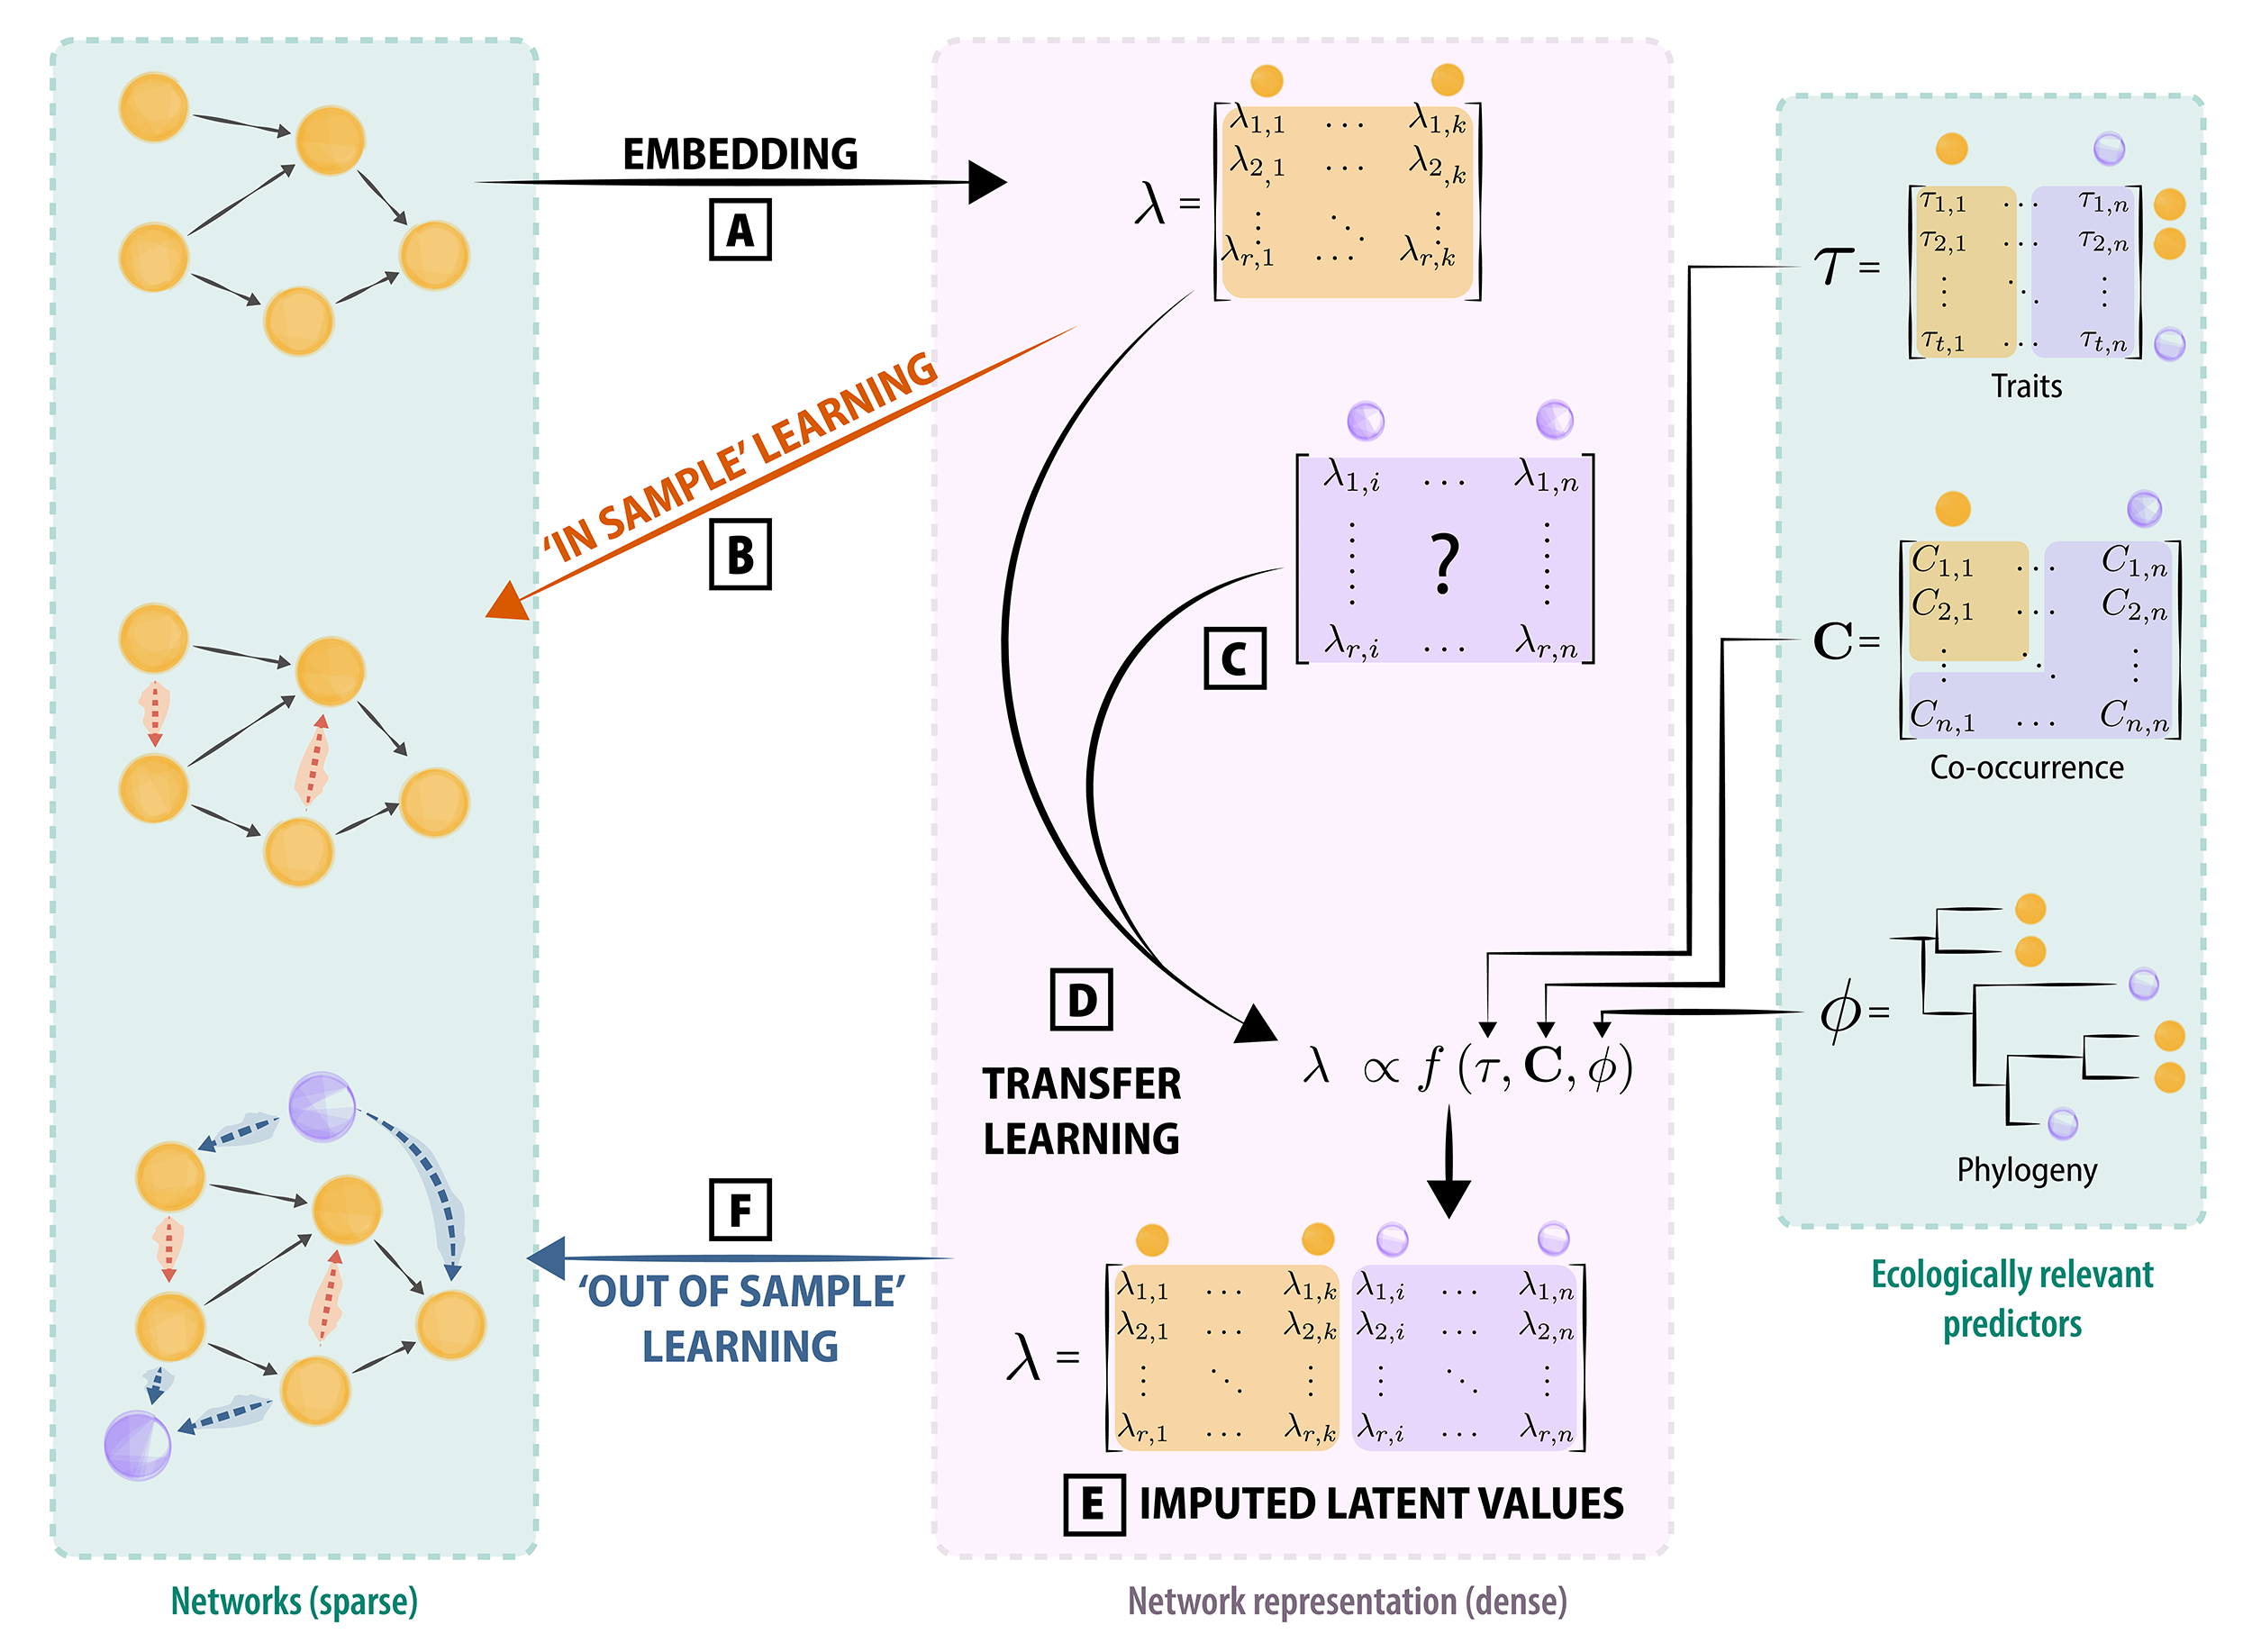
\includegraphics[width=\textwidth]{figures/conceptual_2.png}
    \caption{The embedding process (\textbf{A}) can help to identify links
(interactions) that may have been missed within the original community
(represented by the orange dashed arrows, \textbf{B}). Transfer learning
(\textbf{D}) allows for the prediction links (interactions) even when
novel species (\textbf{C}) are included alongside the original
community. This is achieved by learning using other relevant predictors
(\emph{e.g.,} traits) in conjunction with the known interactions to infer
latent values (\textbf{E}). Ultimately this allows us to predict links
(interactions) for species external from the original sample (blue
dashed arrows) as well as missing within sample links (\textbf{F}).
Within this context the predicted (and original) networks as well as the
ecological predictors used (green boxes) are products that can be
quantified through measurements in the field, whereas the embedded as
well as imputed matrices (purple box) are representative of a
decomposition of the interaction matrices onto the embedding
space}
    \label{fig:embedding}
\end{figure}

\section{Graph embedding offers promises for the inference of potential
interactions}\label{graph-embedding-offers-promises-for-the-inference-of-potential-interactions}

Graph (or network) embedding (\autoref{fig:embedding}) is a family of machine
learning techniques, whose main task is to learn a mapping function from
a discrete graph to a continuous domain (\cite{Arsov2019Network,
Chami2022Machine}). Their main goal is to learn a low dimensional
vector representation of the graph (embeddings), such that its key
properties (\emph{e.g.,} local or global structures) are retained in the
embedding space (\cite{Yan2005Graph}). The embedding space may, but will
not necessarily, have lower dimensionality than the graph. Ecological
networks are promising candidates for the routine application of
embeddings, as they tend to possess a shared structural backbone (see
\emph{e.g.,} \cite{BramonMora2018Identifying}), which hints at structural
invariants in empirical data. Assuming that these structural invariants
are common enough, they would dominate the structure of networks, and
therefore be adequately captured by the first (lower) dimensions of an
embedding, without the need to measure derived aspects of their
structure (\emph{e.g.,} motifs, paths, modularity, \ldots).

\subsection{Graph embedding produces latent variables (but not
traits)}\label{graph-embedding-produces-latent-variables-but-not-traits}

Before moving further, it is important to clarify the epistemic status
of node values derived from embeddings: specifically, they are
\emph{not} functional traits, and therefore should not be interpreted in
terms of effects or responses. As per the framework of
\cite{Malaterre2019Functional}, these values neither derive from, nor result
in, changes in organismal performance, and should therefore not be used
to quantify \emph{e.g.,} functional diversity. This holds true even when
there are correlations between latent values and functional traits:
although these enable an ecological discussion of how traits condition
the structure of the network, the existence of a statistical
relationship does not elevate the latent values to the status of
functional traits.

Rather than directly predicting biological rules (see \emph{e.g.,}
\cite{Pichler2020Machine} for an overview), which may be confounded by the
sparse nature of graph data, learning embeddings works in the
low-dimensional space that maximizes information about the network
structure. This approach is further justified by the observation, for
example, that the macro-evolutionary history of a network is adequately
represented by some graph embeddings (Random dot product graphs
(RDPG); see \cite{DallaRiva2016Exploring}). In a recent publication,
\cite{Strydom2022Food} have used an embedding (based on RDPG) to project a
metaweb of trophic interactions between European mammals, and
transferred this information to mammals of Canada, using the
phylogenetic distance between related clades to infer the values in the
latent subspace into which the European metaweb was projected. By
performing the RDPG step on re-constructed values, this approach yields
a probabilistic trophic metaweb for mammals of Canada based on knowledge
of European species, despite a limited (\(\approx\) 5\%) taxonomic
overlap, and illustrates how the values derived from an embedding can be
used for prediction without being ``traits'' of the species they
represent.

\subsection{Ecological networks are good candidates for
embedding}\label{ecological-networks-are-good-candidates-for-embedding}

Food webs are inherently low-dimensional objects, and can be adequately
represented with less than ten dimensions (\cite{Braga2021Phylogenetic,
Eklof2013Dimensionality, Braga2019Spatial}). Simulation results by
\cite{Botella2022Appraisal} suggested that there is no dominant method to
identify architectural similarities between networks: multiple
approaches need to be tested and compared to the network descriptor of
interest on a problem-specific basis. This matches previous results on
graph embedding, wherein different embedding algorithms yield different
network embeddings (\cite{Goyal2018Graph}), calling for a careful
selection of the problem-specific approach to use. In \autoref{tbl:methods}, we
present a selection of common graph and node embedding methods,
alongside examples of their use to predict interactions or statistical
associations between species. These methods rely largely on linear
algebra or pseudo-random walks on graphs. All forms of embeddings
presented in \autoref{tbl:methods} share the common property of summarizing their
objects into (sets of) dense feature vectors, that capture the overall
network structure, pairwise information on nodes, and emergent aspects
of the network, in a compressed way (\emph{i.e.,} with some information
loss, as we later discuss in the illustration). Node embeddings tend to
focus on maintaining pairwise relationships (\emph{i.e.,} species
interactions), while graph embeddings focus on maintaining the network
structure (\emph{i.e.,} emergent properties). Nevertheless, some graph
embedding techniques (like RDPG, see \emph{e.g.,} \cite{Wu2021Maximum}) will
provide high-quality node-level embeddings while also preserving network
structure.

Graph embeddings \emph{can} serve as a dimensionality reduction method.
For example, RDPG (\cite{Strydom2022Food}) and t-SVD (truncated Singular
Value Decomposition; (\cite{Poisot2021ImpMam}) typically embed networks
using fewer dimensions than the original network (the original network
has as many dimensions as species, and as many informative dimensions as
trophically unique species; \cite{Strydom2021SvdEnt}). However, this is not
necessarily the case -- indeed, one may perform a PCA (a special case of
SVD) to project the raw data into a subspace that improves the efficacy
of t-SNE (t-distributed stochastic neighbor embedding;
\cite{Maaten2009Learning}). There are many dimensionality reductions
(\cite{Anowar2021Conceptual}) that can be applied to an embedded network
should the need for dimensionality reduction (for example for data
visualization) arise. In brief, many graph embeddings \emph{can} serve
as dimensionality reduction steps, but not all do, neither do all
dimensionality reduction methods provide adequate graph embedding
capacities. In the next section (and \autoref{fig:embedding}), we show how the
amount of dimensionality reduction can affect the quality of the
embedding.

\begin{table}[h]
\resizebox{\textwidth}{!}{
\centering
\begin{tabular}{||c c c c c||} 
 \hline
 Method & Object & Technique & Reference & Application \\ [0.2ex] \hline\hline
 tSNE & nodes & statistical divergence & \cite{Hinton2002Stochastic} & 
\vtop{\hbox{\strut \cite{Cieslak2020Tdistributed}, species-environment responses\(^a\)}\hbox{\strut \cite{Gibb2021Data}, host-virus network representation}} \\
LINE & nodes & stochastic gradient descent & \cite{Tang2015Line} & \\
SDNE & nodes & gradient descent & \cite{Wang2016Structural} & \\
node2vec & nodes & stochastic gradient descent & \cite{Grover2016Node2vec}
& \\
HARP & nodes & meta-strategy & \cite{Chen2017Harp} & \\
DMSE & joint nodes & deep neural network & \cite{Chen2017Deep} &
\cite{Chen2017Deep}, species-environment interactions\(^b\) \\
graph2vec & sub-graph & skipgram network & \cite{Narayanan2017Graph2vec} & \\
RDPG & graph & SVD & \cite{Young2007Random} & \vtop{\hbox{\strut \cite{DallaRiva2016Exploring},
trophic interactions}\hbox{\strut \cite{Poisot2021ImpMam}, host-virus network prediction}} \\
GLEE & graph & Laplacian eigenmap & \cite{Torres2020Glee} & \\
DeepWalk & graph & stochastic gradient descent & \cite{Perozzi2014Deepwalk} &
\cite{Wardeh2021Predicting}, host-virus interactions \\
GraphKKE & graph & stochastic differential equation &
\cite{Melnyk2020Graphkke} & \cite{Melnyk2020Graphkke}, microbiome species
associations\(^a\) \\
FastEmbed & graph & eigen decomposition & \cite{Ramasamy2015Compressive} & \\
PCA & graph & eigen decomposition & \cite{Surendran2013Graph} &
\cite{Strydom2021Roadmap}, host-parasite interactions \\
Joint methods & multiple graphs & multiple strategies & \cite{Wang2021Joint}
& \\ [0.2ex]  
 \hline
\end{tabular}
}
\caption{Overview of some common graph embedding approaches, by type of
embedded objects, alongside examples of their use in the prediction of
species interactions. These methods have not yet been routinely used to
predict species interactions; most examples that we identified were
either statistical associations, or analogues to joint species
distribution models. See also Box 1 for an additional discussion on Graph Neural Networks. \(^a\): application is concerned with
\emph{statistical} interactions, which are not necessarily direct
biotic interactions; \(^b\):application is concerned with joint-SDM-like
approach, which is also very close to statistical associations as
opposed to direct biotic interactions. Given the need to evaluate
different methods on a problem-specific basis, the fact that a lot of
methods have not been used on network problems is an opportunity for
benchmarking and method development. Note that the row for PCA also
applies to kernel/probabilistic PCA, which are variations on the more
general method of SVD. Note further that tSNE has been included because
it is frequently used to embed graphs, including of species
associations/interactions, despite not being strictly speaking, a graph
embedding technique (see \emph{e.g.,} \cite{Chami2022Machine}.)}
\label{tbl:methods}
\end{table}

\clearpage

\begin{summary}
\textbf{Graph Neural Networks}

One prominent family of approaches we do not discuss in the present
manuscript is Graph Neural Networks (GNN; \cite{Zhou2020Graph}). GNN are,
in a sense, a method to embed a graph into a dense subspace, but belong
to the family of deep learning methods, which has its own set of
practices (see \emph{e.g.,} \cite{Goodfellow2016Deep}). An important issue with
methods based on deep learning is that, because their parameter space is
immense, the sample size of the data fed into them must be similarly
large (typically thousands of instances). This is a requirement for the
model to converge correctly during training, but this assumption is
unlikely to be met given the size of datasets currently available for
metawebs (or single time/location species interaction networks). This
data volume requirement is mostly absent from the techniques we list
below. Furthermore, GNN still have some challenges related to their
shallow structure, and concerns related to scalability (see
\cite{Gupta2021Graph} for a review), which are mostly absent from the
methods listed in \autoref{tbl:methods}. Assuming that the uptake of
next-generation biomonitoring techniques does indeed deliver larger
datasets on species interactions (\cite{Bohan2017Nextgeneration}), there
is nevertheless the potential for GNN to become an applicable
embedding/predictive technique in the coming years.
\end{summary}

The popularity of graph embedding techniques in machine learning is more
than the search for structural invariants: graphs are discrete objects,
and machine learning techniques tend to handle continuous data better.
Bringing a sparse graph into a continuous, dense vector space
(\cite{Xu2021Understanding}) opens up a broader variety of predictive
algorithms, notably of the sort that are able to predict events as
probabilities (\cite{Murphy2022Probabilistic}). Furthermore, the
projection of the graph itself is a representation that can be learned;
(\cite{Runghen2021Exploiting}), for example, used a neural network to learn the
embedding of a network in which not all interactions were known, based
on the nodes' metadata. This example has many parallels in ecology (see
\autoref{fig:embedding} \textbf{C}), in which node metadata can be represented by
phylogeny, abundance, or functional traits. Using phylogeny as a source
of information assumes (or strives to capture) the action of
evolutionary processes on network structure, which at least for food
webs have been well documented (\cite{Braga2021Phylogenetic,
DallaRiva2016Exploring, Eklof2016Phylogenetic, Stouffer2007Evidence,
Stouffer2012Evolutionary}); similarly, the use of functional traits
assumes that interactions can be inferred from the knowledge of
trait-matching rules, which is similarly well supported in the empirical
literature (\cite{Bartomeus2013Understanding, Bartomeus2016ComFra,
Goebel2023Body, Gravel2013Inferring}). Relating this information to
an embedding rather than a list of network measures would allow to
capture their effect on the more fundamental aspects of network
structure; conversely, the absence of a phylogenetic or functional
signal may suggest that evolutionary/trait processes are not strong
drivers of network structure, therefore opening a new way to perform
hypothesis testing.

\section{An illustration of metaweb
embedding}\label{an-illustration-of-metaweb-embedding}

In this section, we illustrate the embedding of a collection of
bipartite networks collected by \cite{Hadfield2014TalTwo}, using t-SVD and RDPG.
Briefly, an RDPG decomposes a network into two subspaces (left and
right), which are matrices that when multiplied give an approximation of
the original network. RDPG has the particularly desirable properties of
being a graph embedding technique that produces relevant node-level
feature vectors, and provides good approximations of graphs with varied
structures (\cite{Athreya2017Statistical}). The code to reproduce this
example is available as supplementary material in \autoref{supp:perspectives} (note, for the sake of
comparison, that \cite{Strydom2021Roadmap} have an example using embedding
through PCA followed by prediction using a deep neural network on the
same dataset). The resulting (binary) metaweb \(\mathcal{M}\) has 2131
interactions between 206 parasites and 121 hosts, and its adjacency
matrix has full rank (\emph{i.e.,} it represents a space with 121
dimensions). All analyses were done using \texttt{Julia} (\cite{Bezanson2017Julia})
version 1.7.2, \texttt{Makie.jl} (\cite{Danisch2021Makie}), and
\texttt{EcologicalNetworks.jl} (\cite{Poisot2019EcoJl}).

\begin{figure}[h]
    \centering
    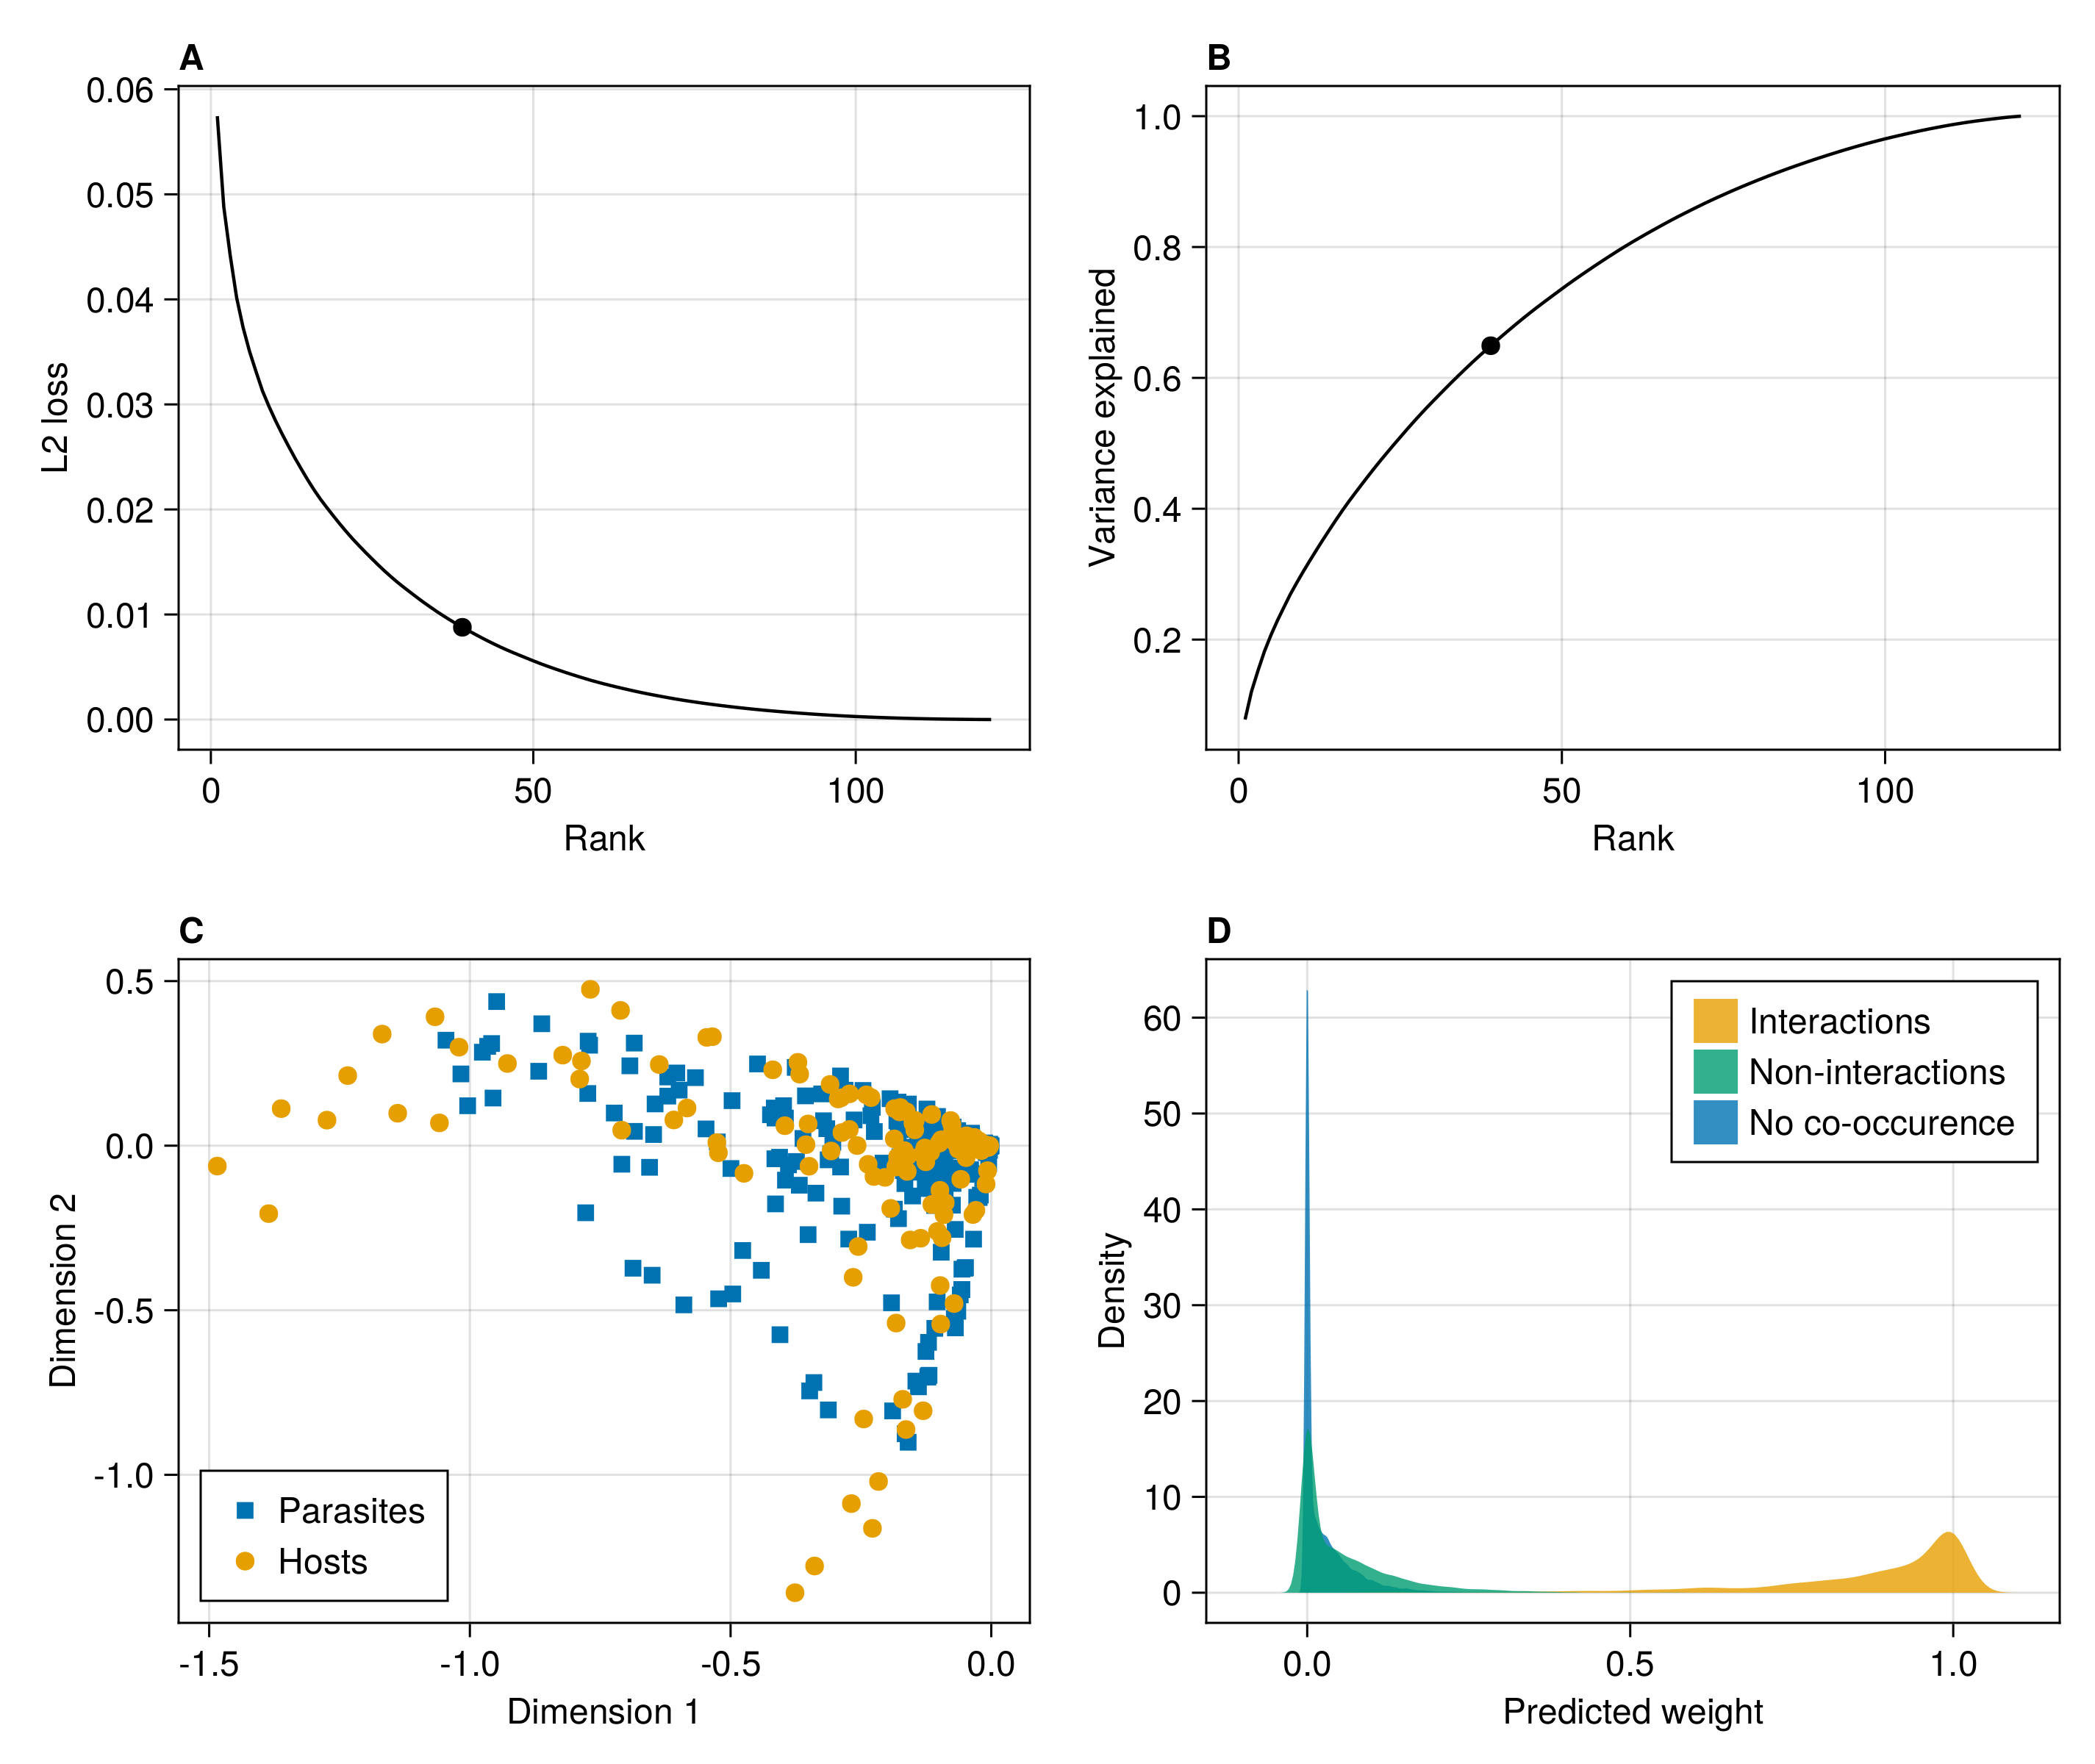
\includegraphics[width=\textwidth]{figures/illustration-part1.png}
    \caption{Validation of an embedding for a host-parasite metaweb, using
Random Dot Product Graphs. \textbf{A}, decrease in approximation error
as the number of dimensions in the subspaces increases. \textbf{B},
increase in cumulative variance explained as the number of ranks
considered increases; in \textbf{A} and \textbf{B}, the dot represents
the point of inflexion in the curve (at rank 39) estimated using the
finite differences method. \textbf{C}, position of hosts and parasites
in the space of latent variables on the first and second dimensions of
their respective subspaces (the results have been clamped to the unit
interval). \textbf{D}, predicted interaction weight from the RDPG based
on the status of the species pair in the
metaweb.}
    \label{fig:illustration1}
\end{figure}

\clearpage

In \autoref{fig:illustration1}, we focus on some statistical checks of the
embedding. In panel \textbf{A}, we show that the averaged \(L_2\) loss
(\emph{i.e.,} the sum of squared errors) between the empirical and
reconstructed metaweb decreases when the number of dimensions (rank) of
the subspace increases, with an inflection at 39 dimensions (out of 120
initially) according to the finite differences method. As discussed by
\cite{Runghen2021Exploiting}, there is often a trade-off between the number of
dimensions to use (more dimensions are more computationally demanding)
and the quality of the representation. In panel \textbf{B}, we show the
increase in cumulative variance explained at each rank, and visualize
that using 39 ranks explains about 70\% of the variance in the empirical
metaweb. This is a different information from the \(L_2\) loss (which is
averaged across interactions), as it works on the eigenvalues of the
embedding, and therefore captures higher-level features of the network.
In panel \textbf{C}, we show positions of hosts and parasites on the
first two dimensions of the left and right subspaces. Note that these
values largely skew negative, because the first dimensions capture the
coarse structure of the network: most pairs of species do not interact,
and therefore have negative values. Finally in panel \textbf{D}, we show
the predicted weight (\emph{i.e.,} the result of the multiplication of
the RDGP subspaces at a rank of 39) as a function of whether the
interactions are observed, not-observed, or unknown due to lack of
co-occurrence in the original dataset. This reveals that the observed
interactions have higher predicted weights, although there is some
overlap; the usual approach to identify potential interactions based on
this information would be a thresholding analysis, which is outside the
scope of this manuscript (and is done in the papers cited in this
illustration). Because the values returned from RDPG are not bound to
the unit interval, we performed a clamping of the weights to the unit
space, showing a one-inflation in documented interactions, and a
zero-inflation in other species pairs. This last figure crosses from the
statistical into the ecological, by showing that species pairs with no
documented co-occurrence have weights that are not distinguishable from
species pairs with no documented interactions, suggesting that (as
befits a host-parasite model) the ability to interact is a strong
predictor of co-occurrence.

\begin{figure}[h]
    \centering
    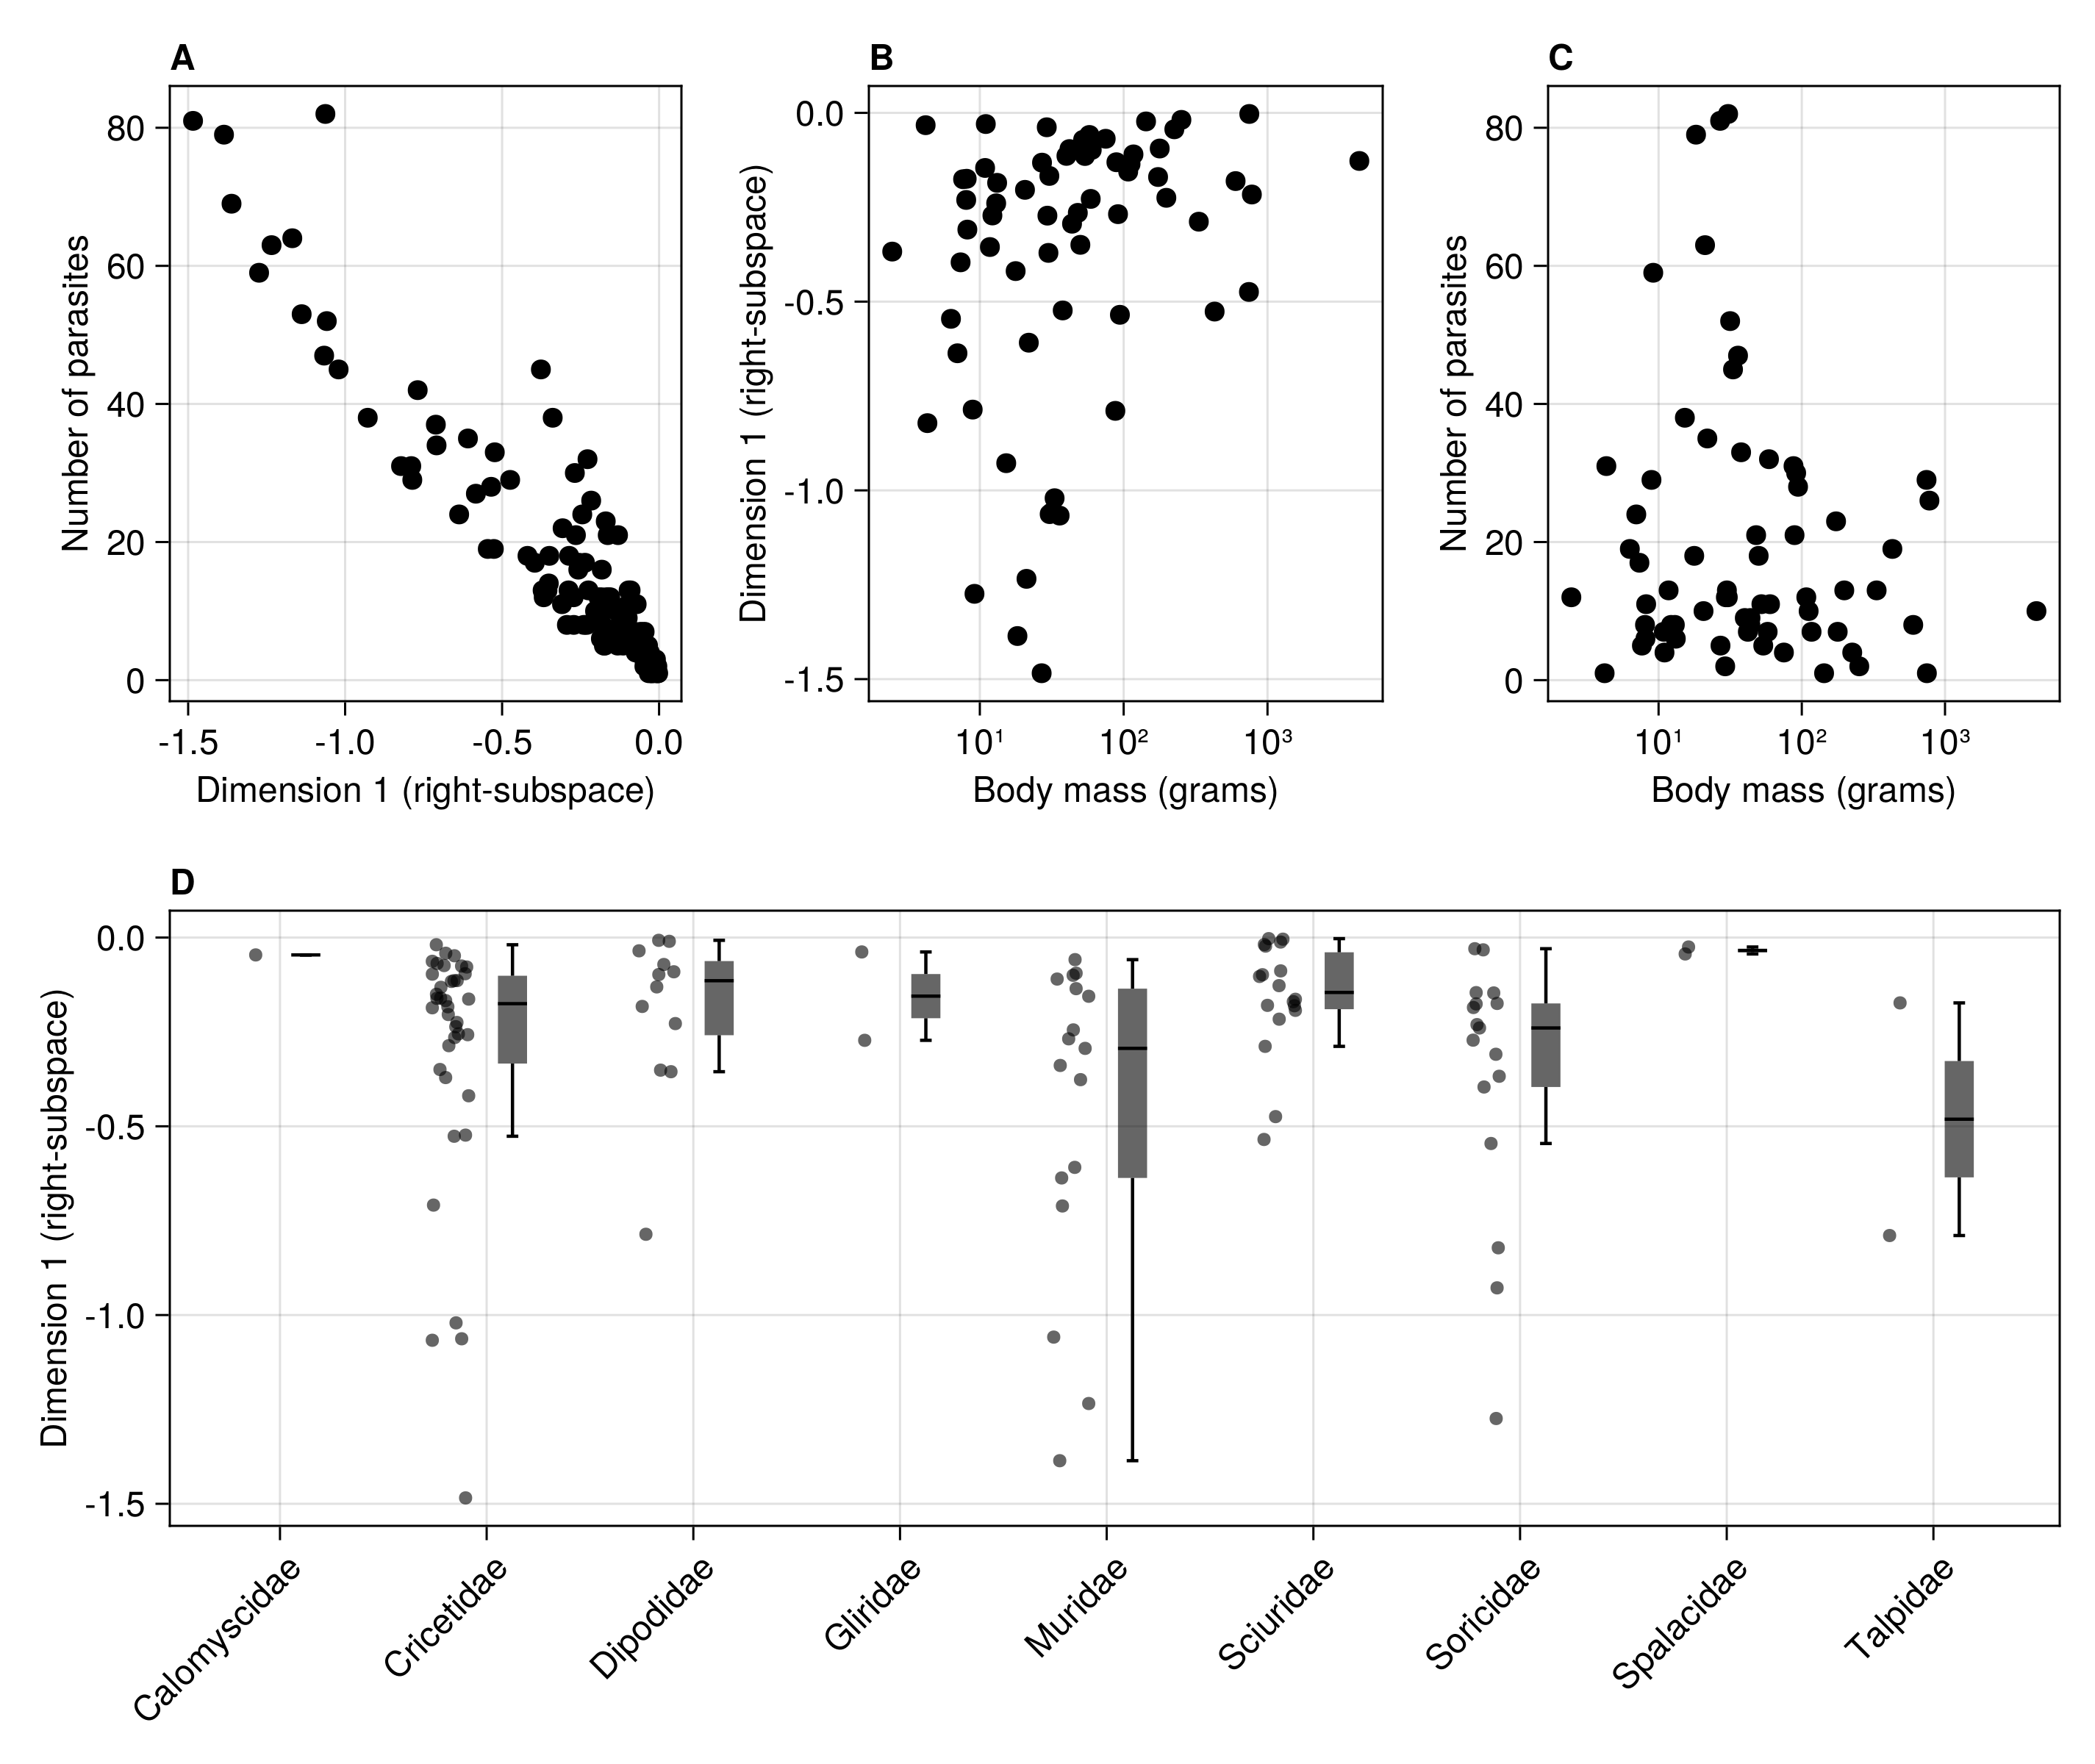
\includegraphics[width=\textwidth]{figures/illustration-part2.png}
    \caption{Ecological analysis of an embedding for a host-parasite
metaweb, using Random Dot Product Graphs. \textbf{A}, relationship
between the number of parasites and position along the first axis of the
right-subspace for all hosts, showing that the embedding captures
elements of network structure at the species scale. \textbf{B}, weak
relationship between the body mass of hosts (in grams) and the position
alongside the same dimension. \textbf{C}, weak relationship between body
mass of hosts and parasite richness. \textbf{D}, distribution of
positions alongside the same axis for hosts grouped by taxonomic
family.}
    \label{fig:illustration2}
\end{figure}

\clearpage

The results of \autoref{fig:illustration1} show that we can extract an embedding
of the metaweb that captures enough variance to be relevant;
specifically, this is true for both \(L_2\) loss (indicating that RDPG
is able to capture pairwise processes) and the cumulative variance
explained (indicating that RDPG is able to capture network-level
structure). Therefore, in \autoref{fig:illustration2}, we relate the values of
latent variables for hosts to different ecologically-relevant data. In
panel \textbf{A}, we show that host with a higher value on the first
dimension have fewer parasites. This relates to the body size of hosts
in the \emph{PanTHERIA} database (\cite{Jones2009Pantheria}), as shown in
panel \textbf{B}: interestingly, the position on the first axis is only
weakly correlated to body mass of the host; this matches well
established results showing that body size/mass is not always a direct
predictor of parasite richness in terrestrial mammals
(\cite{Morand1998Density}), a result we observe in panel \textbf{C}.
Finally, in panel \textbf{D}, we can see how different taxonomic
families occupy different positions on the first axis, with \emph{e.g.,}
Sciuridae being biased towards higher values. These results show how we
can look for ecological informations in the output of network
embeddings, which can further be refined into the selection of
predictors for transfer learning.

\section{The metaweb merges ecological hypotheses and
practices}\label{the-metaweb-merges-ecological-hypotheses-and-practices}

Metaweb inference seeks to provide information about the interactions
between species at a large spatial scale, typically a scale large enough
to be considered of biogeographic relevance (indeed, many of the
examples covered in the introduction span areas larger than a country,
some of them global). But as \cite{Herbert1965Dune} rightfully pointed out,
``[y]ou can't draw neat lines around planet-wide problems''; any
inference of a metaweb must therefore contend with several novel,
interwoven, families of problems. In this section, we outline three that
we think are particularly important, and can discuss how they may
addressed with subsequent data analysis or simulations, and how they
emerge in the specific context of using embeddings; some of these issues
are related to the application of these methods at the science-policy
interface.

\subsection{Identifying the properties of the network to
embed}\label{identifying-the-properties-of-the-network-to-embed}

If the initial metaweb is too narrow in scope, notably from a taxonomic
point of view, the chances of finding another area with enough related
species (through phylogenetic relatedness or similarity of functional
traits) to make a reliable inference decreases. This is because transfer
requires similarity (\autoref{fig:embedding}). A diagnostic for the lack of
similar species would likely be large confidence intervals during
estimation of the values in the low-rank space. In other words, the
representation of the original graph is difficult to transfer to the new
problem. Alternatively, if the initial metaweb is too large
(taxonomically), then the resulting embeddings would need to represent
interactions between taxonomic groups that are not present in the new
location. This would lead to a much higher variance in the starting
dataset, and to under-dispersion in the target dataset, resulting in the
potential under or over estimation of the strength of new predicted
interactions. \cite{Llewelyn2022Predicting} provided compelling evidence for
these situations by showing that, even at small spatial scales, the
transfer of information about interactions becomes more challenging when
areas rich with endemic species are considered. The lack of well
documented metawebs is currently preventing the development of more
concrete guidelines. The question of phylogenetic relatedness and
distribution is notably relevant if the metaweb is assembled in an area
with mostly endemic species (\emph{e.g.,} a system that has undergone
recent radiation or that has remained in isolation for a long period of
time might not have an analogous system with which to draw knowledge
from), and as with every predictive algorithm, there is room for the
application of our best ecological judgement. Because this problem
relates to distribution of species in the geographic or phylogenetic
space, it can certainly be approached through assessing the performance
of embedding transfer in simulated starting/target species pools.

\subsection{Identifying the scope of the prediction to
perform}\label{identifying-the-scope-of-the-prediction-to-perform}

The area for which we seek to predict the metaweb should determine the
species pool on which the embedding is performed. Metawebs can be
constructed by assigning interactions in a list of species within
specific regions. The upside of this approach is that information
relevant for the construction of this dataset is likely to exist, as
countries usually set conservation goals at the national level
(\cite{Buxton2021Key}), and as quantitative instruments are consequently
designed to work at these scales (\cite{Turak2017Using}); specific
strategies are often enacted at smaller scales, nested within a specific
country (\cite{Ray2021Biodiversity}). However, there is no guarantee that
these arbitrary boundaries are meaningful. In fact, we do not have a
satisfying answer to the question of ``where does an ecological network
stop?'', the answer to which would dictate the spatial span to
embed/predict. Recent results by \cite{Martins2022Global} suggested that
networks are shaped within eco-regions, with abrupt structural
transitions from an eco-region to the next. Should this trend hold
generally, this would provide an ecologically-relevant scale at which
metawebs can be downscaled and predicted. Other solutions could leverage
network-area relationships to identify areas in which networks are
structurally similar (see \emph{e.g.,} \cite{Fortin2021Network,
Galiana2018Spatial, Galiana2022Ecological}). Both of these solutions
require ample pre-existing information about the network in space.
Nevertheless, the inclusion of species for which we have data but that
are not in the right spatial extent \emph{may} improve the performance
of approaches based on embedding and transfer, \emph{if} they increase
the similarity between the target and destination network. This proposal
can specifically be evaluated by adding nodes to the network to embed,
and assessing the performance of predictive models (see \emph{e.g.,}
\cite{Llewelyn2022Predicting}).

\section{Conclusion: metawebs, predictions, and
people}\label{conclusion-metawebs-predictions-and-people}

Predictive approaches in ecology, regardless of the scale at which they
are deployed and the intent of their deployment, originate in the
framework that contributed to the ongoing biodiversity crisis
(\cite{Adam2014Elephant}) and reinforced environmental injustice
(\cite{Choudry2013Saving, Dominguez2020Decolonising}). The risk of
embedding this legacy in our models is real, especially when the impact
of this legacy on species pools is being increasingly documented. This
problem can be addressed by re-framing the way we interact with models,
especially when models are intended to support conservation actions.
Particularly on territories that were traditionally stewarded by
Indigenous people, we must interrogate how predictive approaches and the
biases that underpin them can be put to task in accompanying Indigenous
principles of land management (\cite{Eichhorn2019Steps,
Nokmaq2021Awakening}). The discussion of ``algorithm-in-the-loop''
approaches that is now pervasive in the machine learning community
provides examples of why this is important. Human-algorithm interactions
are notoriously difficult and can yield adverse effects
(\cite{Green2019Disparate, Stevenson2021Algorithmic}), suggesting the
need to systematically study them for the specific purpose of, here,
biodiversity governance. Improving the algorithmic literacy of decision
makers is part of the solution (\emph{e.g.,} \cite{Lamba2019Deep, 
MoseboFernandes2020Machine}), as we can reasonably expect that model
outputs will be increasingly used to drive policy decisions
(\cite{Weiskopf2022Increasing}). Our discussion of these approaches need
to go beyond the technical and statistical, and into the governance
consequences they can have. To embed data also embeds historical and
contemporary biases that acted on these data, both because they shaped
the ecological processes generating them, and the global processes
leading to their measurement and publication. For a domain as vast as
species interaction networks, these biases exist at multiple scales
along the way, and a challenge for prediction is not only to develop (or
adopt) new quantitative tools, but to assess the behavior of these tools
in the proper context.

\begin{summary}\label{box:people}
\textbf{Minding legacies shaping ecological datasets}

In large parts of the world, boundaries that delineate geographic
regions are merely a reflection the legacy of settler colonialism, which
drives global disparity in capacity to collect and publish ecological
data. Applying any embedding to biased data does not debias them, but
rather embeds these biases, propagating them to the models using
embeddings to make predictions. Furthermore, the use of ecological data
itself is not an apolitical act (\cite{Nost2021Political}): data
infrastructures tend to be designed to answer questions within national
boundaries (therefore placing contingencies on what is available to be
embedded), their use often drawing upon, and reinforcing, territorial
statecraft (see \emph{e.g.,} \cite{Barrett2005Environment}). As per
\cite{Machen2021Thinking}, these biases are particularly important to consider
when knowledge generated algorithmically is used to supplement or
replace human decision-making, especially for governance (\emph{e.g.,}
enacting conservation decisions on the basis of model prediction). As
information on networks is increasingly leveraged for conservation
actions (see \emph{e.g.,} \cite{Eero2021Use, Naman2022Food,
Stier2017Integrating}), the need to appraise and correct biases that
are unwittingly propagated to algorithms when embedded from the original
data is immense. These considerations are even more urgent in the
specific context of biodiversity data. Long-term colonial legacies still
shape taxonomic composition to this day (\cite{Lenzner2022Naturalized,
Raja2022Colonialism}), and much shorter-term changes in taxonomic and
genetic richness of wildlife emerged through environmental racism
(\cite{Schmidt2022Systemic}). Thus, the set of species found at a specific
location is not only as the result of a response to ecological processes
separate from human influence, but also the result of human-environment
interaction as well as the result legislative/political histories.
\end{summary}

\textbf{Acknowledgements:} We acknowledge that this study was conducted
on land within the traditional unceded territory of the Saint Lawrence
Iroquoian, Anishinabewaki, Mohawk, Huron-Wendat, and Omàmiwininiwak
nations. TP, TS, DC, and LP received funding from the Canadian Institute
for Ecology \& Evolution. FB is funded by the Institute for Data
Valorization (IVADO). TS, SB, and TP are funded by a donation from the
Courtois Foundation. CB was awarded a Mitacs Elevate Fellowship no.
IT12391, in partnership with fRI Research, and also acknowledges funding
from Alberta Innovates and the Forest Resources Improvement Association
of Alberta. M-JF acknowledges funding from NSERC Discovery Grant and
NSERC CRC. RR is funded by New Zealand's Biological Heritage Ngā Koiora
Tuku Iho National Science Challenge, administered by New Zealand
Ministry of Business, Innovation, and Employment. BM is funded by the
NSERC Alexander Graham Bell Canada Graduate Scholarship and the FRQNT
master's scholarship. LP acknowledges funding from NSERC Discovery Grant
(NSERC RGPIN-2019-05771). TP acknowledges financial support from the
Fondation Courtois, and NSERC through the Discovery Grants and Discovery
Accelerator Supplement programs. MJF is supported by an NSERC PDF and an
RBC Post-Doctoral Fellowship.


\printbibliography{}
\end{refsection}

\endinput
%%
%% End of file `article1.tex'.
